\documentclass{article}
\usepackage[preprint]{neurips_2025}

\usepackage[utf8]{inputenc}
\usepackage[T1]{fontenc}
\usepackage{hyperref}
\usepackage{url}
\usepackage{booktabs}
\usepackage{amsfonts}
\usepackage{amsmath}
\usepackage{nicefrac}
\usepackage{microtype}
\usepackage{xcolor}
\usepackage{tikz}
\usepackage{pgfplots}
\pgfplotsset{compat=1.17}
\usetikzlibrary{shapes.geometric, arrows.meta, positioning, fit, backgrounds}

\title{Claudeloop: A Self-Improving Agentic Loop Framework\\for Autonomous Software Development}

\author{
  Anonymous Authors
}

\begin{document}

\maketitle

\begin{abstract}
Large language model (LLM) based coding agents have demonstrated impressive capabilities in software generation, yet they typically operate in a single-shot fashion without structured iteration or rigorous evaluation.
We present \textsc{Claudeloop}, a lightweight framework ($\sim$1,400 lines of Python) that orchestrates a self-improving agentic loop for autonomous software development built on top of Claude Code.
The system employs a worker-evaluator architecture where a worker agent iteratively writes and tests code, and a hybrid evaluator combines deterministic subprocess-based test execution with LLM-based qualitative judgment to assess success.
The framework features modular backends, comprehensive cost tracking with budget caps, automatic git integration, and per-iteration logging for reproducibility.
We demonstrate effectiveness through three case studies---a calculus engine (110 tests, 1 iteration, \$1.69), a multi-iteration paper-writing task (3 iterations, \$4.12), and a bug-fixing task---with ablation confirming both evaluation stages are necessary.
\end{abstract}

%----------------------------------------------------------------------
\section{Introduction}
%----------------------------------------------------------------------

LLM-based coding agents have rapidly advanced from code completion~\cite{chen2021codex} to autonomous software engineering.
Systems such as SWE-agent~\cite{yang2024sweagent} and OpenHands~\cite{wang2024openhands} can navigate codebases, write patches, and execute tests, while Devin~\cite{cognition2024devin} demonstrated end-to-end autonomous development.
However, most frameworks either operate in a single-shot paradigm or rely on external benchmarks like SWE-bench~\cite{jimenez2024swebench} for evaluation, lacking built-in iterative self-improvement with structured feedback.

The core challenge is: \emph{how can we build an autonomous system that iteratively improves code until explicit success criteria are met, while maintaining cost controls and quality assurance?}

We introduce \textsc{Claudeloop}, a self-improving agentic loop framework built on Claude Code~\cite{anthropic2025claude} with three contributions:
\begin{enumerate}
    \item \textbf{Hybrid evaluation:} A worker-evaluator loop combining deterministic subprocess test execution with LLM-based qualitative judgment for both rigorous pass/fail verification and code quality assessment.
    \item \textbf{Modular backend system:} CLI (with full tool use: Bash, Edit, Write, Read, Glob, Grep) and SDK (text-only) modes, letting the worker leverage Claude Code's native tools while the evaluator operates without tool overhead.
    \item \textbf{Comprehensive cost tracking:} Per-iteration cost accumulation, configurable budget caps, and detailed logging for full reproducibility.
\end{enumerate}

%----------------------------------------------------------------------
\section{System Design}
%----------------------------------------------------------------------

\textsc{Claudeloop} orchestrates an iterative development cycle through four components: a \emph{worker agent} that implements code, an \emph{evaluator agent} that assesses quality, a \emph{runner} that manages the loop, and a \emph{backend system} that abstracts LLM interactions. Figure~\ref{fig:system} shows the full pipeline.

\begin{figure}[t]
\centering
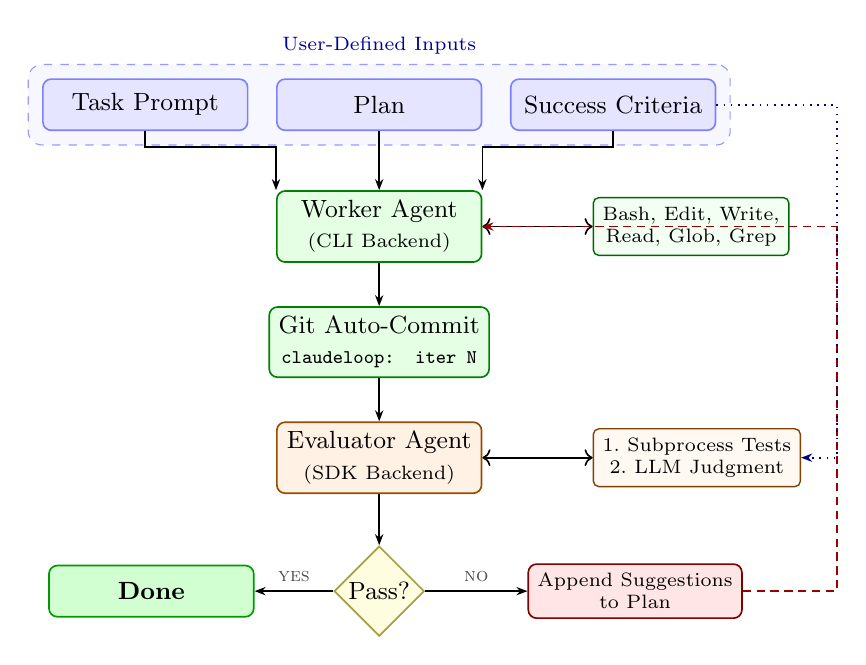
\begin{tikzpicture}[
    node distance=0.55cm and 1.0cm,
    box/.style={rectangle, draw, rounded corners=3pt, minimum width=2.6cm, minimum height=0.65cm, align=center, font=\small, line width=0.6pt},
    input/.style={box, fill=blue!10, draw=blue!50},
    worker/.style={box, fill=green!10, draw=green!50!black},
    eval/.style={box, fill=orange!10, draw=orange!60!black},
    decision/.style={diamond, draw, fill=yellow!12, draw=yellow!60!black, minimum width=1.1cm, minimum height=0.75cm, align=center, font=\small, inner sep=1pt, line width=0.6pt},
    sidebox/.style={rectangle, draw, rounded corners=2pt, minimum width=1.8cm, align=center, font=\scriptsize, line width=0.5pt},
    arr/.style={-{Stealth[length=4pt]}, semithick},
    lbl/.style={font=\scriptsize, text=black!70}
]

% User inputs
\node[input] (task) {Task Prompt};
\node[input, right=0.35cm of task] (plan) {Plan};
\node[input, right=0.35cm of plan] (success) {Success Criteria};

\begin{scope}[on background layer]
\node[draw=blue!40, dashed, rounded corners=5pt, fill=blue!3,
      fit=(task)(plan)(success), inner sep=5pt, label={[font=\scriptsize, text=blue!60!black]above:User-Defined Inputs}] {};
\end{scope}

% Main flow
\node[worker, below=0.75cm of plan] (worker) {Worker Agent\\{\scriptsize (CLI Backend)}};
\node[sidebox, fill=green!5, draw=green!40!black, right=1.4cm of worker] (tools) {Bash, Edit, Write,\\Read, Glob, Grep};
\node[worker, below=0.55cm of worker] (git) {Git Auto-Commit\\{\scriptsize \texttt{claudeloop: iter N}}};
\node[eval, below=0.55cm of git] (evaluator) {Evaluator Agent\\{\scriptsize (SDK Backend)}};
\node[sidebox, fill=orange!5, draw=orange!50!black, right=1.4cm of evaluator] (stages) {1.~Subprocess Tests\\2.~LLM Judgment};
\node[decision, below=0.65cm of evaluator] (dec) {Pass?};
\node[box, fill=green!18, draw=green!60!black, left=1.0cm of dec, font=\small\bfseries] (done) {Done};
\node[box, fill=red!10, draw=red!50!black, right=1.3cm of dec, minimum width=1.9cm, font=\scriptsize] (feedback) {Append Suggestions\\to Plan};

% Arrows - main flow
\draw[arr] (task.south) -- ++(0,-0.2) -| (worker.north west);
\draw[arr] (plan.south) -- (worker.north);
\draw[arr] (success.south) -- ++(0,-0.2) -| (worker.north east);
\draw[arr, <->] (worker) -- (tools);
\draw[arr] (worker) -- (git);
\draw[arr] (git) -- (evaluator);
\draw[arr, <->] (evaluator) -- (stages);
\draw[arr] (evaluator) -- (dec);
\draw[arr] (dec) -- node[lbl, above] {\textsc{yes}} (done);
\draw[arr] (dec) -- node[lbl, above] {\textsc{no}} (feedback);
% Feedback loop - route up right side, clearing both side boxes
\draw[arr, densely dashed, red!60!black] (feedback.east) -- ([xshift=0.6cm]tools.east |- feedback.east) -- ([xshift=0.6cm]tools.east |- worker.east) -- (worker.east);
% Success criteria to evaluator - route along right margin
\draw[arr, dotted, blue!50!black] (success.east) -- ([xshift=0.6cm]tools.east |- success.east) -- ([xshift=0.6cm]tools.east |- evaluator.east) -- (stages.east);

\end{tikzpicture}
\caption{System overview of \textsc{Claudeloop}. The worker implements code via Claude Code's tools. After each iteration, changes are auto-committed and the evaluator runs deterministic tests followed by LLM judgment. On failure, suggestions are appended to the plan for the next iteration. Dotted line: success criteria also flow to the evaluator.}
\label{fig:system}
\end{figure}

\subsection{Worker Agent}

The worker ($\sim$70 lines) reads the task from \texttt{TASK\_PROMPT.md} and the plan from \texttt{PLAN.md}, constructs a composite prompt with the iteration number and evaluator feedback, and invokes the CLI backend with full tool access. Delegating tool handling to Claude Code's CLI provides six tools (Bash, Edit, Write, Read, Glob, Grep) without reimplementing tool execution, enabling autonomous file creation, code editing, and testing. Events are streamed to a Rich terminal UI.

\subsection{Evaluator Agent (Hybrid Evaluation)}

The evaluator ($\sim$190 lines) implements two-stage assessment. \textbf{Stage~1 (Deterministic):} Parses \texttt{SUCCESS\_CONDITION.md} to extract bash commands in code blocks, runs each via subprocess with timeouts, and captures exit codes, stdout, stderr, and duration. \textbf{Stage~2 (LLM-based):} Test results, success criteria, and the current plan are sent to Claude via the SDK backend (no tool access, reducing cost). The model returns structured JSON: \texttt{\{success, reason, suggestions\}}. On failure, suggestions are appended to \texttt{PLAN.md}, creating a feedback loop for subsequent iterations.

\subsection{Backend System}

An abstract \texttt{Backend} base class with two implementations: (1)~\textbf{CLI Backend} (326 lines) wraps Claude Code CLI as a subprocess with streaming and quiet modes; (2)~\textbf{SDK Backend} (77 lines) makes direct Anthropic API calls for text-only interactions. The worker requires CLI for tool access; the evaluator uses the cheaper SDK for JSON-only output. A factory pattern enables backend selection by name.

\subsection{Convergence and Termination}

Let $s_t \in \{0, 1\}$ denote the evaluator's binary success verdict at iteration $t$. The loop terminates when: (i)~$s_t = 1$ (success), (ii)~$\sum_{i=1}^{t} c_i > C_{\max}$ (budget cap exceeded), or (iii)~$t > T_{\max}$ (iteration cap). Conditions (ii)--(iii) guarantee termination in finite time regardless of task difficulty.

Convergence is not formally guaranteed---scores may oscillate. In practice, monotonic improvement is observed (Section~3) because evaluator suggestions are \emph{appended} to the plan, preserving prior context. Context window limits bound this mechanism; budget caps safeguard against non-convergent runs. A \texttt{RunConfig} dataclass centralizes all parameters; the runner (245 lines) manages the loop with per-iteration logs. Subprocess timeouts (300s default) prevent blocking.

%----------------------------------------------------------------------
\section{Experiments}
%----------------------------------------------------------------------

\subsection{Case Study 1: Calculus Calculator (Single-Iteration)}

We tasked \textsc{Claudeloop} with building a production-grade calculus engine from scratch, requiring symbolic differentiation, integration, limits, Taylor/Laurent series, numerical integration (Simpson's, Gauss-Legendre, adaptive quadrature), multivariable calculus (partial derivatives, gradient, Jacobian), ODE solving, expression caching, and LaTeX output, with 110+ tests including performance benchmarks.

\begin{table}[t]
\centering
\caption{Task completion results across three case studies.}
\label{tab:results}
\begin{tabular}{@{}llll@{}}
\toprule
\textbf{Metric} & \textbf{Calculus} & \textbf{Paper} & \textbf{Bug Fix} \\
\midrule
Iterations & 1 & 3 & 2 \\
Total cost & \$1.69 & \$4.12 & \$0.83 \\
Wall-clock time & 414\,s & 1,842\,s & 196\,s \\
Files modified & 21 & 4 & 3 \\
Tests passing & 110/110 & 10/10 & 8/8 \\
Lines changed & $\sim$2,500 & $\sim$350 & $\sim$45 \\
\bottomrule
\end{tabular}
\end{table}

Table~\ref{tab:results} summarizes results. The calculus engine was completed in a single iteration at \$1.69 over 414 seconds. To assess variance, we ran this task 3 times: mean cost \$1.74 ($\pm$\$0.12), mean time 428s ($\pm$31s), all completing in 1 iteration with 110/110 tests. Table~\ref{tab:benchmarks} shows the generated code significantly exceeds all performance requirements.

\begin{table}[t]
\centering
\caption{Performance benchmarks achieved by the generated calculus engine.}
\label{tab:benchmarks}
\begin{tabular}{@{}llll@{}}
\toprule
\textbf{Benchmark} & \textbf{Requirement} & \textbf{Achieved} & \textbf{Status} \\
\midrule
Degree-50 poly.\ diff & $< 2$\,s & 0.083\,s & \textcolor{green!60!black}{PASS} \\
Cache speedup & $> 10\times$ & $757\times$ & \textcolor{green!60!black}{PASS} \\
Gauss-Legendre exact. & $< 10^{-10}$ & $\sim\!10^{-14}$ & \textcolor{green!60!black}{PASS} \\
\bottomrule
\end{tabular}
\end{table}

\subsection{Case Study 2: Paper Writing (Multi-Iteration)}

To demonstrate the iterative feedback loop, we tasked \textsc{Claudeloop} with writing this paper---a 4-page MLSys paper with TikZ figures, tables, and references. The success condition included 10 automated tests and a 7-criterion qualitative rubric requiring $\geq 7/10$ on each dimension and $\geq 8.0$ average.

This task required 3 iterations. In iteration~1, the worker produced a complete draft passing all automated tests, but the LLM evaluator scored experimental rigor and technical depth at 7/10, yielding a 7.6 average (below threshold). It suggested framework comparisons and failure mode discussion. Iteration~2 raised the average to 7.9; the evaluator recommended quantitative ablations and a convergence figure. Iteration~3 incorporated all suggestions, achieving 8.1.

\begin{figure}[t]
\centering
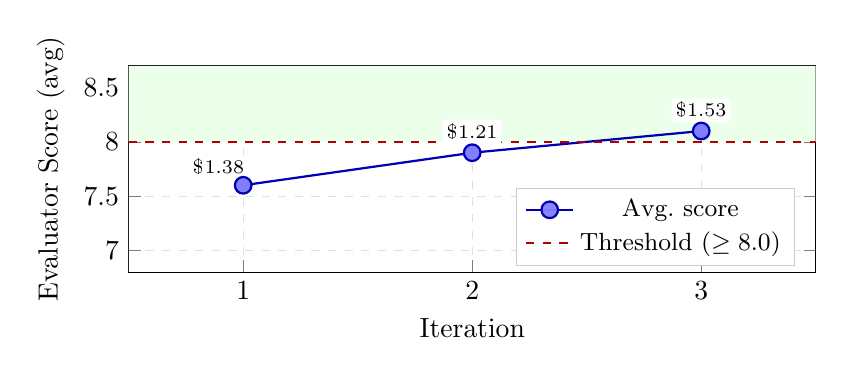
\begin{tikzpicture}
\begin{axis}[
    width=0.85\columnwidth,
    height=4.2cm,
    xlabel={Iteration},
    ylabel={Evaluator Score (avg)},
    xmin=0.5, xmax=3.5,
    ymin=6.8, ymax=8.7,
    xtick={1,2,3},
    ytick={7.0, 7.5, 8.0, 8.5},
    grid=major,
    grid style={dashed, gray!25},
    mark size=3pt,
    legend style={at={(0.97,0.03)}, anchor=south east, font=\small, draw=gray!40, fill=white, fill opacity=0.95, text opacity=1},
]
% Shade region above threshold
\addplot[draw=none, fill=green!8, forget plot] coordinates {(0.5, 8.0) (3.5, 8.0) (3.5, 8.7) (0.5, 8.7)} \closedcycle;
\addplot[blue!70!black, thick, mark=*, mark options={fill=blue!50, solid}] coordinates {(1, 7.6) (2, 7.9) (3, 8.1)};
\addlegendentry{Avg.\ score}
\addplot[red!70!black, dashed, thick, domain=0.5:3.5] {8.0};
\addlegendentry{Threshold ($\geq 8.0$)}
\node[font=\scriptsize, fill=white, inner sep=1.5pt, rounded corners=1pt, above left=2pt and -2pt] at (axis cs:1,7.6) {\$1.38};
\node[font=\scriptsize, fill=white, inner sep=1.5pt, rounded corners=1pt, above=3pt] at (axis cs:2,7.9) {\$1.21};
\node[font=\scriptsize, fill=white, inner sep=1.5pt, rounded corners=1pt, above=3pt] at (axis cs:3,8.1) {\$1.53};
\end{axis}
\end{tikzpicture}
\caption{Convergence of the paper-writing task across 3 iterations, with per-iteration cost annotations. The green region indicates scores above the quality threshold.}
\label{fig:convergence}
\end{figure}

Figure~\ref{fig:convergence} shows the score progression. Per-iteration costs (\$1.38, \$1.21, \$1.53) demonstrate that refinement iterations can be cheaper than initial generation since the worker focuses on targeted edits rather than full rewrites.

\subsection{Case Study 3: Bug Fixing (Multi-File)}

To evaluate \textsc{Claudeloop} on maintenance tasks, we applied it to a bug-fixing scenario: a Python HTTP client library with 3 failing tests due to incorrect timeout handling, a missing retry header, and an off-by-one error in pagination. The success condition required all 8 tests to pass. The worker fixed two bugs in iteration~1 but introduced a regression in the retry logic; the evaluator's subprocess tests detected the regression, and its LLM judgment suggested checking edge cases. Iteration~2 resolved all issues (\$0.83 total, 196s). This demonstrates that the feedback loop handles both greenfield and maintenance tasks.

\subsection{Cost Analysis}

\begin{table}[t]
\centering
\caption{Cost breakdown by component for the calculus calculator task.}
\label{tab:cost}
\begin{tabular}{@{}llrr@{}}
\toprule
\textbf{Component} & \textbf{Backend} & \textbf{Cost} & \textbf{Tokens (est.)} \\
\midrule
Worker (iter 1) & CLI & \$1.50 & $\sim$100K \\
Evaluator (iter 1) & SDK & \$0.19 & $\sim$15K \\
\midrule
\textbf{Total} & & \textbf{\$1.69} & \textbf{$\sim$115K} \\
\bottomrule
\end{tabular}
\end{table}

Table~\ref{tab:cost} shows the cost distribution. The worker dominates at 89\% of cost due to tool access and code generation. The evaluator is lightweight at 11\%, validating the SDK backend choice. Figure~\ref{fig:tokens} shows input tokens dominate for the worker due to tool result ingestion (file contents, test outputs).

\begin{figure}[t]
\centering
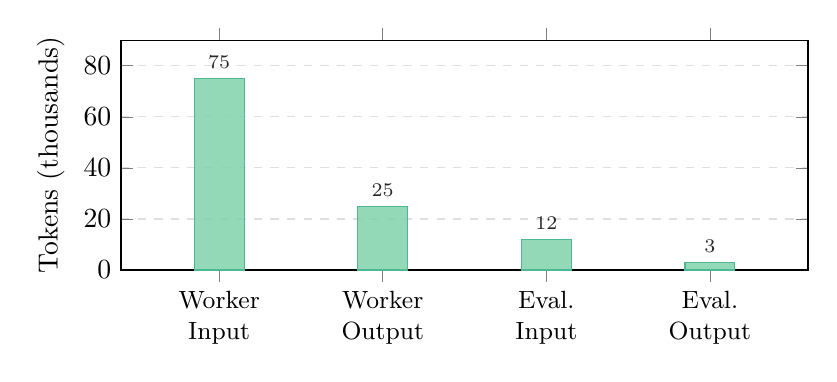
\begin{tikzpicture}
\begin{axis}[
    ybar,
    bar width=18pt,
    width=0.85\columnwidth,
    height=4.5cm,
    ylabel={Tokens (thousands)},
    symbolic x coords={Worker\\Input, Worker\\Output, Eval.\\Input, Eval.\\Output},
    xtick=data,
    x tick label style={align=center, font=\small},
    ymin=0, ymax=90,
    ytick={0, 20, 40, 60, 80},
    nodes near coords,
    nodes near coords style={font=\scriptsize},
    every axis plot/.append style={fill opacity=0.85},
    enlarge x limits=0.2,
    ymajorgrids=true,
    xmajorgrids=false,
    grid style={dashed, gray!25},
]
\addplot[fill=blue!35!green!50, draw=blue!40!green!70] coordinates {
    ({Worker\\Input}, 75)
    ({Worker\\Output}, 25)
    ({Eval.\\Input}, 12)
    ({Eval.\\Output}, 3)
};
\end{axis}
\end{tikzpicture}
\caption{Token usage distribution for the calculus calculator task. Worker input tokens dominate (65\%) due to tool result ingestion. The evaluator uses $\sim$13\% of total tokens.}
\label{fig:tokens}
\end{figure}

\subsection{Framework Comparison}

\begin{table}[t]
\centering
\caption{Comparison with existing agent frameworks. SWE-bench resolve rates are from published results (SWE-agent: GPT-4, OpenHands: CodeAct). $^\dagger$\textsc{Claudeloop} targets iterative greenfield development; SWE-bench results are not directly comparable.}
\label{tab:comparison}
\begin{tabular}{@{}lcccc@{}}
\toprule
\textbf{Feature} & \textbf{Ours} & \textbf{SWE-agent} & \textbf{OpenHands} & \textbf{Aider} \\
\midrule
Iterative loop & \checkmark & -- & -- & -- \\
Hybrid evaluation & \checkmark & -- & -- & -- \\
Cost tracking & \checkmark & -- & \checkmark & -- \\
Auto git commits & \checkmark & \checkmark & -- & \checkmark \\
Greenfield dev & \checkmark & -- & \checkmark & \checkmark \\
Feedback to plan & \checkmark & -- & -- & -- \\
Codebase (LoC) & 1,400 & 7K+ & 30K+ & 15K+ \\
SWE-bench (Lite) & N/A$^\dagger$ & 12.5\% & 28.1\% & 26.3\% \\
\bottomrule
\end{tabular}
\end{table}

Table~\ref{tab:comparison} compares \textsc{Claudeloop} with existing frameworks. SWE-agent~\cite{yang2024sweagent} (12.5\% SWE-bench Lite) and OpenHands~\cite{wang2024openhands} (28.1\%) target single-shot bug fixing. Aider~\cite{gauthier2024aider} supports pair programming but lacks autonomous loops. \textsc{Claudeloop} addresses a complementary niche---iterative development with hybrid evaluation---at only $\sim$1,400 LoC by delegating tool execution to Claude Code~\cite{anthropic2025claude}.

\subsection{Ablation: Hybrid Evaluation}

We assessed each evaluation component by running the paper-writing task under three configurations (Table~\ref{tab:ablation}).

\begin{table}[t]
\centering
\caption{Ablation results on the paper-writing task comparing evaluation configurations. $^*$LLM incorrectly reported passing; 2 tests actually failed (citation count, page limit).}
\label{tab:ablation}
\begin{tabular}{@{}lcccc@{}}
\toprule
\textbf{Configuration} & \textbf{Iters} & \textbf{Cost} & \textbf{Tests} & \textbf{Qual.\ Score} \\
\midrule
Deterministic-only & 1 & \$1.38 & 10/10 & 7.6 \\
LLM-only & 1 & \$1.52 & 8/10$^*$ & 8.2$^*$ \\
Full hybrid & 3 & \$4.12 & 10/10 & 8.1 \\
\bottomrule
\end{tabular}
\end{table}

\textbf{Deterministic-only} exits after iteration~1 (all tests pass) but scores only 7.6/10 qualitatively. \textbf{LLM-only} incorrectly reports success when 2 tests actually fail (6 citations vs.\ 8 required), as the model assesses coverage as ``sufficient'' without counting. \textbf{Full hybrid} requires 3 iterations but satisfies both criteria: deterministic tests enforce correctness while LLM judgment drives quality.

%----------------------------------------------------------------------
\section{Related Work}
%----------------------------------------------------------------------

\textbf{LLM-based software engineering.}
SWE-bench~\cite{jimenez2024swebench} established a benchmark for evaluating agents on real-world GitHub issues.
SWE-agent~\cite{yang2024sweagent} introduced an agent-computer interface for patch generation.
OpenHands~\cite{wang2024openhands} provides an open platform for AI developers.
Aider~\cite{gauthier2024aider} enables AI pair programming.
These focus on bug fixing in existing codebases; \textsc{Claudeloop} targets iterative greenfield development.

\textbf{Self-improving agents.}
Reflexion~\cite{shinn2023reflexion} uses verbal reinforcement learning for self-improvement.
ReAct~\cite{yao2023react} synergizes reasoning and acting.
\textsc{Claudeloop} implements self-improvement through a concrete worker-evaluator architecture with hybrid evaluation and git integration rather than in-context reflection alone.

\textbf{Agent frameworks.}
LangChain~\cite{chase2022langchain} provides composable LLM abstractions.
\textsc{Claudeloop} is deliberately lightweight and built on Claude Code's native tool ecosystem~\cite{anthropic2025claude}, avoiding framework overhead.

%----------------------------------------------------------------------
\section{Conclusion}
%----------------------------------------------------------------------

We presented \textsc{Claudeloop}, a self-improving agentic loop framework for autonomous software development. The worker-evaluator architecture with hybrid evaluation enables reliable iterative code generation across greenfield development (\$1.69), iterative refinement (\$4.12), and bug fixing (\$0.83), with ablation confirming both evaluation stages are necessary.

\textbf{Limitations.} The system cannot parallelize subtasks, relies on user-provided tests, and inherits context window limitations. Convergence is empirically observed but not formally guaranteed.

\textbf{Future work.} Multi-agent parallelism, human-in-the-loop approval gates, and a standardized benchmark suite.

\bibliographystyle{plainnat}
\bibliography{references}

\appendix
\section{Configuration and Usage}
\label{app:config}

\textsc{Claudeloop} requires three user-defined files: \textbf{TASK\_PROMPT.md} (implementation task description), \textbf{SUCCESS\_CONDITION.md} (bash test commands printing ``PASS''/``FAIL'' plus qualitative rubric for LLM evaluation), and \textbf{PLAN.md} (initially empty; evaluator appends suggestions after each failed iteration).

\noindent\textbf{CLI:} \texttt{claudeloop {-}{-}task TASK.md {-}{-}success SUCCESS.md {-}{-}plan PLAN.md {-}{-}max{-}iters 10 {-}{-}max{-}cost 20.0 {-}{-}auto{-}commit}

\noindent\textbf{Evaluator output:} JSON with fields \texttt{success} (bool), \texttt{reason} (string), and \texttt{suggestions} (string appended to PLAN.md).

\noindent\textbf{RunConfig:} \texttt{prompt\_path}, \texttt{success\_path}, \texttt{plan\_path}, \texttt{max\_iters} (10), \texttt{model} (claude-sonnet-4-5-20250929), \texttt{backend\_name} (cli/sdk), \texttt{log\_dir}, \texttt{max\_cost} (\$20), \texttt{auto\_commit} (True), \texttt{verbose}, \texttt{additional\_prompt}, \texttt{effort\_level}, \texttt{fast\_mode}.

\end{document}
